%%%%%%%%%%%%%%%%%%%%%%%%%%%%%%%%%%%%%%%%%%%%%%%%%%%%%%%%%%%%%%%%%%%%%%%%%%%%%%%%
% SD Lab -- Containers
% Giovanni Ciatto
% Alma Mater Studiorum - Università di Bologna
% mailto:giovanni.ciatto@unibo.it
%%%%%%%%%%%%%%%%%%%%%%%%%%%%%%%%%%%%%%%%%%%%%%%%%%%%%%%%%%%%%%%%%%%%%%%%%%%%%%%%
%\documentclass[handout]{beamer}\mode<handout>{\usetheme{default}}
%
\documentclass[presentation]{beamer}\mode<presentation>{\usetheme{AMSBolognaFC}}
%\documentclass[handout]{beamer}\mode<handout>{\usetheme{AMSBolognaFC}}
%%%%%%%%%%%%%%%%%%%%%%%%%%%%%%%%%%%%%%%%%%%%%%%%%%%%%%%%%%%%%%%%%%%%%%%%%%%%%%%%
\usepackage{sd-lab-common}
\usepackage{sd-lab-containers}
%%%%%%%%%%%%%%%%%%%%%%%%%%%%%%%%%%%%%%%%%%%%%%%%%%%%%%%%%%%%%%%%%%%%%%%%%%%%%%%%
\title[\currentLab{} -- Containers 101]{Containers 101}
%
\subtitle{\courseName{} (\courseAcronym) / Module \moduleN{}}
%
\author[\sspeaker{\gcShort} \& \mmShort]{
	\speaker{\gcFull} \and \mmFull
	\\ 
	\gcEmail \and \mmEmail
}
%
\institute[\disiShort, \uniboShort]{\disi{} (\disiShort)\\\unibo}
%
\date[A.Y. \academicYear{}]{Academic Year \academicYear{}}
%
%%%%%%%%%%%%%%%%%%%%%%%%%%%%%%%%%%%%%%%%%%%%%%%%%%%%%%%%%%%%%%%%%%%%%%%%%%%%%%%%
\begin{document}
%%%%%%%%%%%%%%%%%%%%%%%%%%%%%%%%%%%%%%%%%%%%%%%%%%%%%%%%%%%%%%%%%%%%%%%%%%%%%%%%

%/////////
\frame{\titlepage}
%/////////

%%===============================================================================
\section*{Outline}
%%===============================================================================
%
%%/////////
\frame[c]{\tableofcontents[hideallsubsections]}
%%/////////

\section{Motivation}

\begin{frame}
\frametitle{Lecture goals}

    \begin{itemize}
        \item In this course, you may need a way to reproduce Lab exercises on your personal computers, possibly simulating a distributed environment

        \vfill{}

        \item Furthermore, you must be able to submit your homeworks/projects being sure they will run on other computer too
        \begin{itemize}
            \item Avoiding the situation \emph{``No, I swear, it used to work on my PC''} :)

            \item[!] Making your results more durable and \alert{reproducible}
        \end{itemize}

        \vfill{}

        \item You will learn some fundamentals of:
        \begin{itemize}
            \item[$\checkmark$] Build \& automation systems (e.g. \href{https://gradle.org/}{Gradle})
            \item[$\rightarrow$] Container Engines (e.g. \href{https://www.docker.com/}{Docker})
        \end{itemize}

        \vfill{}

        \item By reading \cite{envConf}, you can easily:
        \begin{itemize}
            \item[$\checkmark$] install Docker on your personal PC
            \item[$\rightarrow$] register a Docker ID with your \texttt{@studio.unibo.it} email address
        \end{itemize}
    \end{itemize}

\end{frame}

\section{Containers}

\begin{frame}
    \frametitle{Bare metal vs. VM vs. Containers}

    \begin{center}
        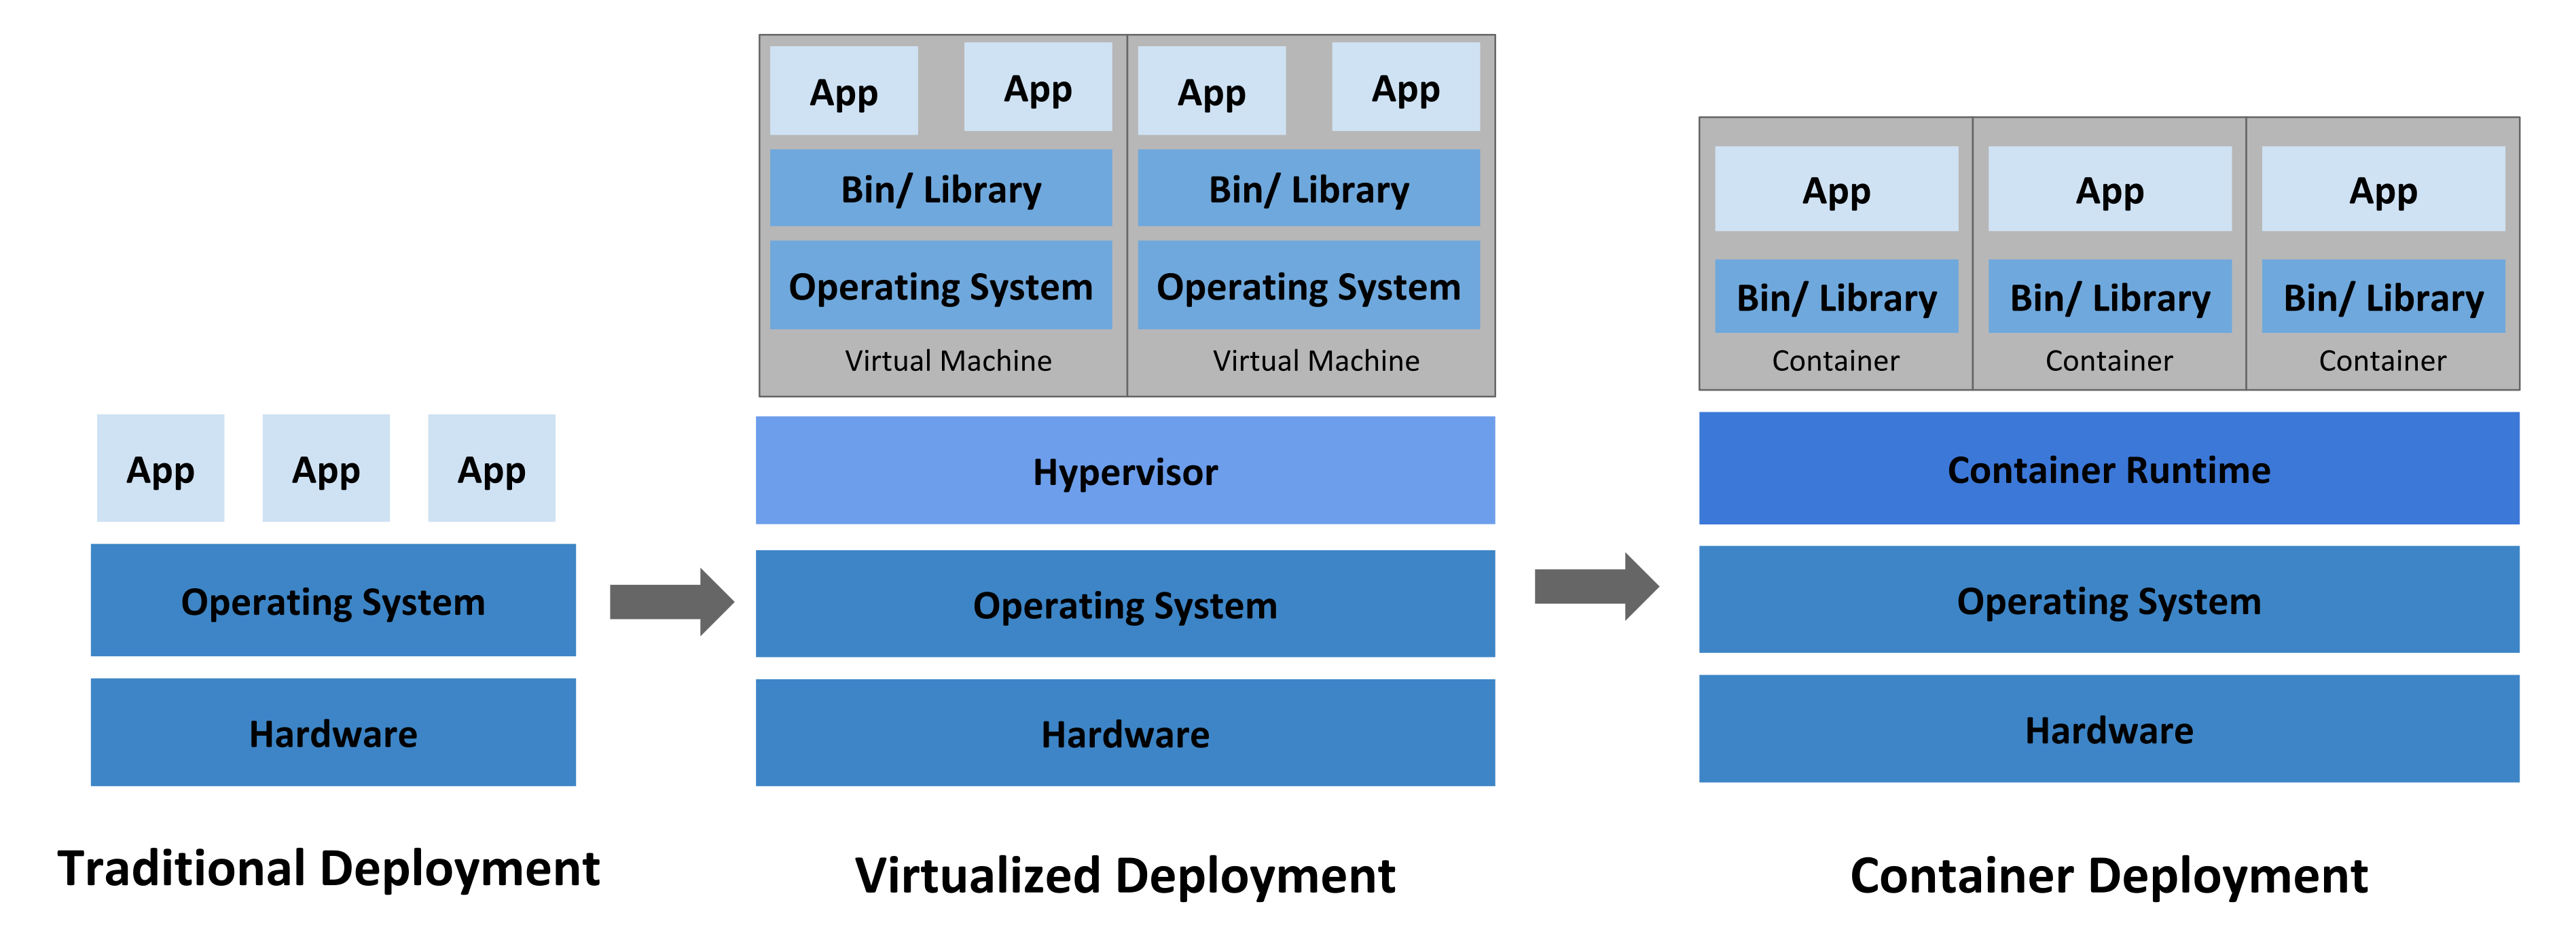
\includegraphics[width=\linewidth]{figures/vm-vs-containers.png}
    \end{center}

\end{frame}

\begin{frame}
\frametitle{Containers}

    \begin{block}{}
        Containers are \alert{lightweight} virtual machines usually \emph{wrapping} a \alert{single application} and along with its \alert{environment}---there including environment variables, configuration files, network facilities, runtimes and operating systems. They can be deployed and transferred as a whole
    \end{block}
    %
    \begin{itemize}
        \item They are deployable on any machine hosting a \alert{container engine}
        %
        \begin{itemize}\small
            \item such a machine is called \alert{host}
        \end{itemize}

        \item They are \alert{lightweight} as they share the host's kernel \& resources

        \item They are \alert{ephemeral} (storage \& side effects are discarded on end)
%        %
%        \begin{itemize}\small
%            \item[ie] storage and side-effects are discarded upon termination
%        \end{itemize}

        \item Each container is an instance of some \alert{image}:
        %
        \begin{equation*}\small
            \mathit{object} : \mathit{class} = \mathit{container} : \mathit{image}
        \end{equation*}

        \item Images are serialisable and versioned and they are usually shared by means of public \alert{repositories}
    \end{itemize}

\end{frame}

\begin{frame}[allowframebreaks]
    \frametitle{Collateral aspects}

    \begin{block}{Several aspects must be \textbf{virtualised} to support containers' operation}
        \begin{description}
            \item[networks] and \alert{network interfaces}, as well as IP addresses, and host names, and TCP/UDP ports
            %
            \begin{itemize}\small
                \item to support communication among containers over the Internet or LAN \dots
                \item \ldots as if each container is a single machine
            \end{itemize}

            \item[volumes] and \alert{storage facilities}, as well as file systems
            %
            \begin{itemize}\small
                \item to support each container has a fresh new environment\ldots
                \item \ldots isolated from the host and other containers
            \end{itemize}
        \end{description}
    \end{block}

    \begin{block}{Several abstractions can be \textbf{built} on top of containers}
        \begin{description}
            \item[services] --- one or more functionally equivalent containers cooperating in serving requests from a single entry point

            \item[stacks] --- a collection of one or more services composed to provide higher-level facilities
        \end{description}
    \end{block}

\end{frame}

\subsection{Why containers}

\begin{frame}
\frametitle{Why containers}

    \begin{itemize}
        \item We will exploit containers to easily deploy our software

        \item So will you, for your projects, if possible

        \item You may also use containers to simulate a distributed application on a single machine

        \item Containers are the building blocks of \alert{stacks}, which in turn are managed by \alert{orchestrators}, to deploy (\alert{micro})\alert{services}.
        This is what happens, for instance, behind the scenes of a \alert{Cloud} provider

    \end{itemize}

    \bigskip

    \begin{block}{}
        \alert{From now on}, you are \alert{encouraged} to use containers to submit your projects
    \end{block}

\end{frame}

\subsection{Docker}

\begin{frame}[allowframebreaks]
\frametitle{Docker in a Nutshell}

    \begin{block}{Docker is our \textbf{container engine} of choice}
        \begin{itemize}
            \item since it is the leading technology in this field
            \item it works uniformly on most common OS
            \item relatively simple to install and use (w.r.t. competitors)
        \end{itemize}
    \end{block}

    \begin{block}{Similar technologies}
        \begin{itemize}
            \item Kubernetes --- \url{https://kubernetes.io}
            \item Artifactory Docker Registry.
            \item LXC
            \item Hyper-V and Windows Containers.
            \item rkt
            \item Podman
            \item CRI+O
        \end{itemize}
    \end{block}
    %
    \framebreak
    %
    General architecture:
    %
    \begin{center}
        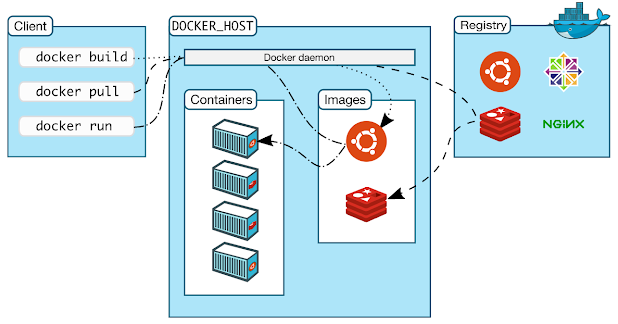
\includegraphics[width=.8\linewidth]{figures/client-vs-daemon.png}
    \end{center}

    \framebreak

    \begin{block}{General command structure}
        \centering\ttfamily

        docker \alert{<resource>} \textit{<command>} <args>
    \end{block}
    %
    where
    %
    \begin{description}\small
        \item[\texttt{resource}] may be \texttt{container}, \texttt{image}, \texttt{service}, \texttt{volume}, etc.
        \item[\texttt{command}] depends on the resource
        \item[\texttt{args}] depend on the command
    \end{description}
    %
    \begin{itemize}\small
        \item[!] for some common commands the resource may be omitted since it's obvious
    \end{itemize}

    \framebreak

    \begin{itemize}

        \item Docker assumes images are \alert{built} out of an existing application by means of \alert{\texttt{Dockefile}s}

        \begin{itemize}
            \item Think about an image as a shut-down OS where a single application -- along with all its dependencies -- is installed
        \end{itemize}

        \smallskip

        \item Containers can be instantiated (i.e. \alert{run}) out of some pre-existing image by invoking a program which is assumed to be installed on that image

        \begin{itemize}
            \item Think about the instantiation process as turning on the OS and invoking that application
        \end{itemize}

        \smallskip

        \begin{center}
            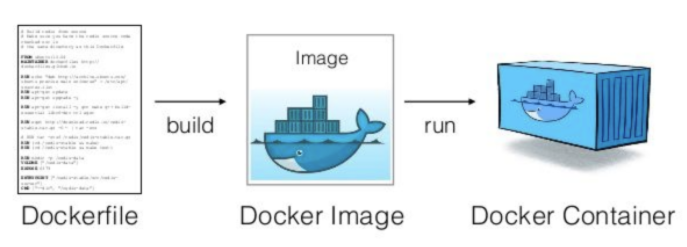
\includegraphics[width=.5\linewidth]{figures/build-run-workflow.png}
        \end{center}

        \framebreak

        \item Volumes, as well as networks, can be specified upon container instantiation
        %
        \begin{itemize}
            \item provided that they have been previously defined
            \item default choices are smart so that users may ignore these aspects most of the time
        \end{itemize}

        \bigskip

        \item Services, stacks, and higher level abstractions are managed via ad-hoc components:
        %
        \begin{itemize}
            \item such as Docker \alert{Compose} (cf. slide \ref{frame:compose}) or Docker \alert{Swarm} (cf. slide \ref{frame:swarm})
        \end{itemize}

    \end{itemize}

\end{frame}

\subsubsection{Images}

\begin{frame}
\frametitle[Docker Images]{Docker Images\hint{Image $\neq$ Picture}}

\begin{itemize}
	\item Images are executable files which, if run, instantiate a container
	\item Usually, you do not manipulate images directly: your local Docker installation takes care of pulling/pushing them from/to an online \alert{repository} for you:
	%
	\begin{itemize}
		\item[\$] \texttt{docker image} \texttt{\alert{<cmd>}}
	\end{itemize}
	%
	where \texttt{<cmd>} may be one of the following:
	%
	\begin{description}
		\item[\texttt{build}] --- builds an image from a \alert{Dockerfile}
		\item[\texttt{ls}] --- lists all locally available images
		\item[\texttt{pull}] --- pulls an image from a \alert{repository} (you must be logged)
		\item[\texttt{push}] --- push an image to a \alert{repository} (you must be logged)
		\item[\texttt{rm}] --- remove one or more images
		\item[\texttt{tag}] --- creates a symbolic tag for an image
		\item[\texttt{--help}] --- shows the list of available commands for images

	\end{description}

\end{itemize}

\end{frame}

\begin{frame}
\frametitle{Docker Images -- Example}
	\begin{enumerate}
		\item Check the list of images currently available on your local machine (you may have none if you are running Docker for the first time)
		\begin{itemize}
		    \item[\$] \texttt{docker image \alert{ls}}
		\end{itemize}

		\item Download (or \alert{pull}) the \href{https://hub.docker.com/_/alpine/}{\texttt{alpine}} image from the Internet
		\begin{itemize}
		    \item[\$] \texttt{docker [image] \alert{pull} \textit{alpine}}
		    \item[] \hint{\texttt{[optional\_term] within square brackets}}
		    \item Where is the image being downloaded from?
		    \begin{itemize}
		        \item The default registry from \url{https://hub.docker.com}, you are assumed to have an account on there
		        \item thus, you own a repository too \texttt{https://hub.docker.com/u/\alert{<your\_username>}}
		    \end{itemize}
		    \item What's \texttt{alpine}?
		    \begin{itemize}
		        \item Alpine Linux\footnote{\url{https://alpinelinux.org/about}} is one of the most lightweight Linux distribution ever
		    \end{itemize}
		\end{itemize}

		\item Re-check the currently available images
		\begin{itemize}
		    \item[\$] \texttt{docker image \alert{ls}}
	    \end{itemize}
	\end{enumerate}
\end{frame}

\subsubsection{Containers}

\begin{frame}[allowframebreaks]
\frametitle{Docker Containers}

\begin{itemize}
    \item Docker containers can be instantiated by means of the following syntax:
    %
    \begin{itemize}
        \item[\$] \texttt{docker [container] \alert{run} [\alert{<opts>}] \alert{\textit{<image>}} [\alert{<cmd>} [\textit{\alert{<args>}}]]}
    \end{itemize}
    %
    where :
    \begin{description}
        \item[\texttt{\textit{<image>}}] is the image to be instantiated,
        \item[\texttt{<cmd>}] is the command to be executed on the container, once instantiated (optional)
        \item[\texttt{\textit{<args>}}] is a sequence of space-separated arguments for \texttt{<cmd>}
        \item[\texttt{<opts>}] is a possibly empty sequence of options for the container instantiation. Several are available.
    \end{description}

    \framebreak

    \item We will only exploit the following options in this lesson:
    %
    \begin{description}\small
        \item[\texttt{-i}] --- runs the container in \emph{\alert{i}nteractive} mode

        \item[\texttt{-t}] --- runs the container in \emph{\alert{t}erminal} emulation mode

        \item[\texttt{-d}] --- runs the container in \emph{\alert{d}aemon} mode \hint{daemons = services}

        \item[\texttt{--rm}] --- \emph{\alert{r}e\alert{m}oves} the container after it terminates

        \item[\texttt{-e \textit{<key>}=<value>}] --- sets an \emph{\alert{e}nvironment} variable \texttt{\textit{<key>}} to \texttt{<value>} on the container, before \texttt{<cmd>} is invoked

        \item[\texttt{-p \textit{<host>}:<guest>}] --- \emph{\alert{p}ublish} port \texttt{<guest>} on the container to port \texttt{\textit{<host>}} on the host

        \item[\texttt{-h \textit{<hostname>}}]  ---  sets the \emph{\alert{h}ostname} of the container to \texttt{\textit{<hostname>}}

        \item[\texttt{-v \textit{<host path>}:<guest path>}]  ---  mounts the host's \texttt{\textit{<host path>}} on the container, into \texttt{<guest path>}, as a \emph{\alert{v}olume}

        \item[\texttt{--name \textit{<name>}}]  ---  assigns a unique \emph{\alert{n}ame} to the container
    \end{description}

    \framebreak

    \item As soon as \texttt{<cmd>} terminates its execution, the container is teminated too and any side effect applied to its storage is reverted

    \medskip

    \item If your application (\texttt{<cmd>}) requires NO user interaction and it CAN just run in the background, you must run it in daemon mode, otherwise in interactive mode

    \medskip

    \item In interactive mode, the application's \texttt{stdin}, \texttt{stdout}, \texttt{stderr} are redirected to/from your console
    %
    \begin{itemize}
        \item this is necessary if the containerised applicationion need to consume the users' inputs
    \end{itemize}

    \medskip

    \item If you need to interact with some container's shell, you should run it in terminal emulation mode
\end{itemize}

\end{frame}

\begin{frame}[allowframebreaks]
\frametitle{Docker Containers -- Example}

    \begin{enumerate}
        \item Run a shell on a novel \texttt{alpine} container, in interactive mode
        %
        \begin{itemize}
            \item[\$] \texttt{docker run -i -e MY\_MSG="Hello World!" alpine sh}
            \begin{itemize}
                \item No, Docker is not freezed :)
                \item You simply started a \alert{very minimal} shell
            \end{itemize}
        \end{itemize}

        \vfill

        \item To convince your self you are within a tiny Linux VM, try running
        %
        \begin{itemize}
            \item[\$] \texttt{cd ; whoami ; pwd ; hostname ; echo \$MY\_MSG}
        \end{itemize}

        \vfill

        \item Cool. What else can a raw Alpine Linux do? Is even Java installed?
        %
        \begin{itemize}
            \item[\$] \texttt{java -version ; javac -version}
        \end{itemize}

        \vfill

        \item No, Java? So bad. Containers have access to the internet (if the guest does too), so you can install software on them
        %
        \begin{itemize}
            \item[\$] \texttt{apk update ; apk add openjdk11} \hint{\href{https://wiki.alpinelinux.org/wiki/Alpine_Linux_package_management}{APK doc here}}
            \item[\$] \texttt{java -version ; javac -version}
        \end{itemize}

        \framebreak

        \item Try now to gracefully terminate the shell
        %
        \begin{itemize}
            \item[\$] \texttt{exit}
            \begin{itemize}
                \item the process launched by \texttt{docker run} terminated, so the container will be terminated too
            \end{itemize}
        \end{itemize}

        \item Re-run the same shell in terminal emulation mode
        %
        \begin{itemize}
            \item[\$] \texttt{docker run \alert{-t} -i -e MY\_MSG="Hello World!" alpine sh}
            \begin{itemize}
                \item Can you see the effect of option \texttt{-t}?
            \end{itemize}
        \end{itemize}

        \item Re-check whether Java is installed or not
        \begin{itemize}
            \item what do you expect?
        \end{itemize}

        \framebreak

        \item \alert{Before terminating this second container}, open another shell \alert{on the host} and run
        %
        \begin{itemize}
            \item[\$] \texttt{docker \alert{ps}}
            \begin{itemize}
                \item this command shows all \alert{currently} running containers
                \item you should be able to spot a line representing your container's info---there including a funny auto-generated name
            \end{itemize}
        \end{itemize}

        \item Try now to check for non-running containers too
        %
        \begin{itemize}
            \item[\$] \texttt{docker ps \alert{-a}}
            \begin{itemize}
                \item can you spot the previous container, the one you installed Java in?
            \end{itemize}
        \end{itemize}

        \item Terminate all containers, gracefully and then delete them all by running
        %
        \begin{itemize}
            \item[\$] \texttt{docker container \alert{prune}}
            \begin{itemize}
                \item now your environment is clean
            \end{itemize}
        \end{itemize}

    \end{enumerate}

\end{frame}

\subsubsection{Dockerfiles}

\begin{frame}%[allowframebreaks]
\frametitle{Dockerfiles}

    Dockerfiles\footnote{Lang reference: \url{https://docs.docker.com/engine/reference/builder}} are scripts aimed at \alert{building} new images
    %
    \begin{enumerate}
        \item An image is built by firstly specifying a \emph{base} image to start \alert{FROM}
        %
        \begin{itemize}
            \item in the simplest cases this is just a raw image such as \texttt{alpine} or \texttt{ubuntu}
            \item but serveral base images are available for most common runtimes, e.g. \href{https://hub.docker.com/r/anapsix/alpine-java/}{\texttt{alpine-java}} or \href{https://hub.docker.com/_/python/}{\texttt{python}}
        \end{itemize}
        \item Some files may be optionally \alert{COPY}ed on the novel image, at specific locations
        \item You can then specify some commands to be \alert{RUN} on the base image to install your application
        \item Some \alert{ENV}ironment variable may be optionally set
        \item Some transport-level port may be optionally \alert{EXPOSE} to the host or to the other containers
        \item Some default \alert{CMD} may optionally be configured to be invoke by default upon container start

    \end{enumerate}

\end{frame}

\startDemo
\begin{frame}[allowframebreaks]
\frametitle{Dockerfiles -- Demo \currentDemo: JEcho Dockerization}

    \begin{exampleblock}{This example is on GitLab as well}
        \begin{itemize}\small
            \item \url{\gitlabRepo}
            %
            \begin{itemize}
                \item look at \texttt{jecho/README.md}
            \end{itemize}
        \end{itemize}
    \end{exampleblock}

    \framebreak

    \begin{enumerate}

        \item Consider the JEcho application from the previous lab
        %
        \begin{itemize}
            \item an echo application with upper- and lower-case modalities
            \item adequately Gradlefied to start via \alert{\texttt{gradle(w) run}}
            \item altered to greet the user mentioned by the \alert{\texttt{JECHO\_USER}} env. var.
        \end{itemize}

        \framebreak

        \item Create a new file named \alert{\texttt{Dockerfile}} within the project root directory (i.e. \alert{\texttt{jecho}}), containing the following lines:
        %
        \lstinputlisting[language=docker]{./listings/Dockerfile1}

        \framebreak

        \item Build the new image by executing the following command:
        %
        \begin{itemize}
            \item[\$] \texttt{docker \alert{build} -t <DockerID>/jecho \alert{.}}\hint{pay attention to the dot}
            \begin{itemize}
                \item where \texttt{DockerID} is your username on \href{https://hub.docker.com/}{Dockerhub}
                \item and \alert{\texttt{<DockerID>/jecho}} is a \alert{tag} for the newly created image
            \end{itemize}
        \end{itemize}

        \item Now have a look to the list of available images on your computer
        %
        \begin{itemize}
            \item[\$] \texttt{docker image ls}
        \end{itemize}

        \item Can you spot the new entry? You can instantiate it as a \alert{named} container by typing
        %
        \begin{itemize}
            \item[\$] \texttt{docker run -t -i \alert{--name jecho} <DockerID>/jecho}
        \end{itemize}

        \item Run the app until it terminates. Can you understand how inputs can be provided to containerised applications?

        \framebreak

        \item From now on, you can re-run the \alert{same} container by typing
        %
        \begin{itemize}
            \item[\$] \texttt{docker [container] \alert{start} -i -a jecho}
        \end{itemize}

        \item Assuming you own an account on \href{https://hub.docker.com/}{DockerHub}, and your local Docker is properly \emph{logged in}, you can now \alert{push} your newly created image by typing
        %
        \begin{itemize}
            \item[\$] \texttt{docker [image] \alert{push} <DockerID>/jecho}
        \end{itemize}

        \item Now everybody can \alert{pull} your image for using it. You can try with your colleagues ones by typing
        %
        \begin{itemize}
            \item[\$] \texttt{docker [image] \alert{pull} <Colleague-DockerID>/jecho}
            \begin{itemize}
                \item What a great way to distribute software! :)
            \end{itemize}
        \end{itemize}

    \end{enumerate}

\end{frame}

%\section{Suggested Exercises}
%
%\begin{frame}%[allowframebreaks]
%\frametitle{Suggested Exercises}
%
%\begin{block}{Dockerify JEcho}
%    Try to Dockerify the JEcho application from previous Labs
%\end{block}
%
%\vfill{}
%
%\begin{block}{Dockerify \textsc{Linda} Service}
%    Try to Dockerify the \textsc{Linda} Service from previous Labs
%\end{block}
%
%\end{frame}

\section{About Docker Compose}

\begin{frame}[allowframebreaks]
    \frametitle{Docker Compose Functionalities}
    \label{frame:compose}

    \begin{itemize}
        \item It is quite common that a number of containers must be (un)deployed \alert{together \& orderly}

        \bigskip

        \item Compose helps users in doing so, via three main ingredients:
        %
        \begin{description}\small
            \item[\texttt{docker-compose.yaml}] files\footnotemark --- which \emph{declaratively} \alert{specifies} which containers should be instantiated, how, and in which order
            \item[\texttt{docker-compose up}] command --- which \alert{instantiates} a \texttt{docker-compose.yaml} file, starting up all containers therein defined, in an orderly fashion
            \item[\texttt{docker-compose down}] command --- which gracefully \alert{disposes} the containers, defined into the local \texttt{docker-compose.yaml} specification
        \end{description}

        \bigskip

        \item Compose usually requires an ad-hoc plugin to be installed in your Docker engine

    \end{itemize}

    \footnotetext{\url{https://docs.docker.com/compose/compose-file}}

    \bigskip

    \begin{exampleblock}{Example about these aspects are provided on GitLab}
        \begin{itemize}\small
            \item \url{\gitlabRepo}
            %
            \begin{itemize}
                \item look at \texttt{hit-counter/README.md} and \texttt{my-blog/README.md} 
            \end{itemize}
        \end{itemize}
    \end{exampleblock}

\end{frame}

\section{About Docker Swarm}

\begin{frame}[allowframebreaks]
    \frametitle{Docker Swarm Functionalities}
    \label{frame:swarm}

    \begin{itemize}
        \item Docker engines may be run in \emph{Swarm} mode
        %
        \begin{itemize}
            \item[\$] \texttt{docker swarm init{\color{gray}|join}}
        \end{itemize}

        \bigskip

        \item Swarms are \alert{clusters} of machines running \emph{federated} Docker engines
        %
        \begin{itemize}
            \item nodes may be added to the cluster dynamically
            \item container may be executed/replicated on several nodes
        \end{itemize}

        \bigskip

        \item In Swarm mode, Docker engines support more functionalities:
        %
        \begin{description}
                \item[services] --- possibly \alert{replicated} servers with automatic load distribution
%            \item[networks] --- virtual networks shared by serveral containers or services
            \item[stacks] --- ensembles of services which must be deployed together, possibly in an orderly fashion
        \end{description}

        \framebreak

        \item Swarm enables \alert{cluster administration}, via three main ingredients:
        %
        \begin{description}\small
            \item[\texttt{docker-compose.yaml}] same syntax and purpose as in Docker Compose: describing stacks of services (each one consisting of one or more containers)
            \item[\texttt{docker stack deploy}] command --- which \alert{instantiates} a \texttt{docker-compose.yaml} stack, starting up all the services there in contained, possibly \alert{spreading them into the cluster}
            \item[\texttt{docker stack rm}] command --- which gracefully \alert{disposes} a stack, given its name
        \end{description}
    \end{itemize}

    \bigskip

    \begin{exampleblock}{Example about these aspects are provided on GitLab}
        \begin{itemize}\small
            \item \url{\gitlabRepo}
            %
            \begin{itemize}
                \item look at \texttt{hit-counter/README.md} and \texttt{hit-counter2/README.md} 
            \end{itemize}
        \end{itemize}
    \end{exampleblock}

\end{frame}

% \subsection{A Java Echo application}

% \startExercise
% \begin{frame}[allowframebreaks]
% \frametitle{Exercise \currentExercise: Java Echo application}

%     \begin{enumerate}
%         \item Clone the Lab-2 GitLab repository at \url{\gitlabGroup/lab-2}
%         %
%         \begin{itemize}
%             \item it stores the Java Echo application within the \texttt{jecho} directory
%             \item which is a simple project: bare Java sources
%             \item the \texttt{im} directory is for the next exercise
%         \end{itemize}

%         \vspace{.5cm}

%         \item Inspect the Java Echo application source code and try to figure out its functioning
%         %
%         \begin{itemize}
%             \item what's its purpose from the user perspective?
%             \item does it requires some arguments? does they affect the application behaviour?
%             \item which assumptions (about the environment) does it relies upon?
%             \item[!] notice that the application requires network communication to occur on port 8080
%         \end{itemize}

%         \framebreak

%         \item Gradlefy the cloned application, making it compilable and runnable by means of \texttt{gradlew}
%         %
%         \begin{itemize}
%             \item you can \alert{generate} a Gradle Wrapper script by means of the following command:
%             %
%             \begin{itemize}
%                 \item[\$] \texttt{gradle wrapper}\hint{\href{https://docs.gradle.org/current/userguide/gradle_wrapper.html}{see Reference here}}
%             \end{itemize}


%             \item other files must be created manually :)

%             \item the canonical directory structure must be created manually :))

%             \item use \alert{environment variables} or Gradle properties to provide arguments to the application

%         \end{itemize}

%         \vspace{.5cm}

%         \item Dockerify the cloned application, creating an image out of it
%         %
%         \begin{itemize}
%             \item notice the application can run in two modes: either \emph{daemon} or \emph{gate}
%             %
%             \begin{itemize}
%                 \item you may need to actually create two images, one for each mode
%             \end{itemize}

%             \item remember to \alert{expose} the 8080 port! \hint{\href{https://docs.docker.com/engine/reference/builder/\#expose}{Reference here}}

%             \item remember to tag the images with the \texttt{\textit{<DockerID>}/jecho-daemon} and \texttt{\textit{<DockerID>}/jecho-gate} tags
%         \end{itemize}

%         \framebreak

%         \item Run the newly created images as containers, named \texttt{jecho-d} and \texttt{jecho-g} respectively
%         %
%         \begin{itemize}
%             \item in case of \texttt{jecho-d}, remember to \alert{publish} the container's 8080 port on the host's 8888 port \hint{\href{https://docs.docker.com/engine/reference/commandline/run/\#options}{Reference here}}

%             \item in case of \texttt{jecho-g}, it need to be provided with the IP of \texttt{jecho-d}

%             \item you can \alert{inspect} a container in order to find its IP:
%             %
%             \begin{itemize}
%                 \item[\$] \texttt{docker container \alert{inspect} jecho-d} \hint{\href{https://docs.docker.com/engine/reference/commandline/container_inspect/}{Reference here}}
%             \end{itemize}

%         \end{itemize}

%         \vspace{.5cm}

%         \item Try interacting with \texttt{jecho-d}, both from the host and from \texttt{jecho-g}

%         \vspace{.5cm}

%         \item Describe your tests into the \texttt{README.md} file
%     \end{enumerate}


% \end{frame}

% \subsection{IM application}

% \startExercise
% \begin{frame}%[allowframebreaks]
% \frametitle{Exercise \currentExercise: IM application, again}

%     \begin{enumerate}
%         \item Gradlefy the IM application from Lab-1
%         %
%         \begin{itemize}
%             \item use environment variables to provide arguments
%             \item store the source code within the \texttt{im} directory
%             \item you can use the provided solution to the Lab-1 exercise, if you didn't completed it
%         \end{itemize}

%         \item Dockerify it

%         \item Instantiate at least 2 containers, each one wrapping an instance of the IM application
%         %
%         \begin{itemize}
%             \item inter-connect them by means of containers' IPs
%         \end{itemize}

%         \item Use 2 disjoint consoles to emulate a multi-IM scenario

%         \item Describe your tests into the \texttt{README.md} file

%         \vspace{1cm}

%         \item[!] Congrats! You are emulating a distributed system on your local PC! :)
%     \end{enumerate}

% \end{frame}

%===============================================================================
\section*{}
%===============================================================================
\frame{\titlepage}

%===============================================================================
% \section*{\bibname}
%===============================================================================

\setbeamertemplate{page number in head/foot}{}
%\\\\\\\\\\\\\\\\\\\\\
%\begin{frame}[t,allowframebreaks,noframenumbering]{\refname}
\begin{frame}[c]{\refname}
    %	\footnotesize
    	\scriptsize
    %\tiny
    \bibliographystyle{plain}
    \bibliography{sd-lab-containers}
\end{frame}
%\\\\\\\\\\\\\\\\\\\\\

%%%%%%%%%%%%%%%%%%%%%%%%%%%%%%%%%%%%%%%%%%%%%%%%%%%%%%%%%%%%%%%%%%%%%%%%%%%%%%%
\end{document}
%%%%%%%%%%%%%%%%%%%%%%%%%%%%%%%%%%%%%%%%%%%%%%%%%%%%%%%%%%%%%%%%%%%%%%%%%%%%%%%%
